\chapter{Estado del Arte}\label{chapter:state-of-the-art}

Dentro de los tipos de sistemas electorales se encuentran dos grandes grupos: los sistemas de pluralidad y los sistemas de mayor\'ia. 

Los sistemas de pluralidad son aquellos en los que el ganador es el candidato que obtiene el mayor n\'umero de votos. Bajo este  criterio, si un candidato $A$ obtiene $40$ votos y dos candidatos $B$ y $C$ obtienen $30$ votos cada uno, entonces gana $A$, aun cuando $60$ votantes (la mayor\'ia) no votaron a su favor. 

En los sistemas de mayor\'ia, por otro lado, es necesario que un candidato alcance la mayor\'ia de votos (un determinado porcentaje de los votos) para obtener la victoria. Si esto no sucede, entonces se decide el ganador mediante un \textit{ranking} o en posteriores rondas de votaci\'on. \todo{@audit ref}

En los sistemas de \textit{ranking}, los electores deben otorgarle un puesto a cada candidato (primero, segundo, tercero, etc.).  Para determinar el ganador, se utilizan m\'etodos como el \textit{desempate instant\'aneo} (IRV, por ``instant-runoff voting'' en ingl\'es). \todo{@audit ref}

\section{M\'etodo del Desempate Instant\'aneo}\label{sec:irv}
En IRV se cuentan los votos de la primera elecci\'on de cada votante. Si un candidato posee m\'as de la mitad de  los votos, entonces gana la elecci\'on. En otro caso, se elimina uno de los candidatos con el menor n\'umero de votos y se le aumenta un voto a la siguiente opci\'on disponible de todos aquellos que hayan elegido al candidato eliminado en primera opci\'on. Esto \'ultimo puede ser visto como que en toda boleta donde el $i$-\'esimo candidato sea el eliminado, el \textit{ranking} se desplaza, esto es, el $(i+1)$-\'esimo pasa a ser el $i$-\'esimo, el $(i+2)$-\'esimo pasa a ser el $(i+1)$-\'esimo, etc\'etera. El proceso contin\'ua hasta que alg\'un candidato obtenga m\'as de la mitad de los votos. 

La figura \ref{fig:irv} muestra el diagrama de flujo del IRV.

\begin{figure}[!h]
    \centering
    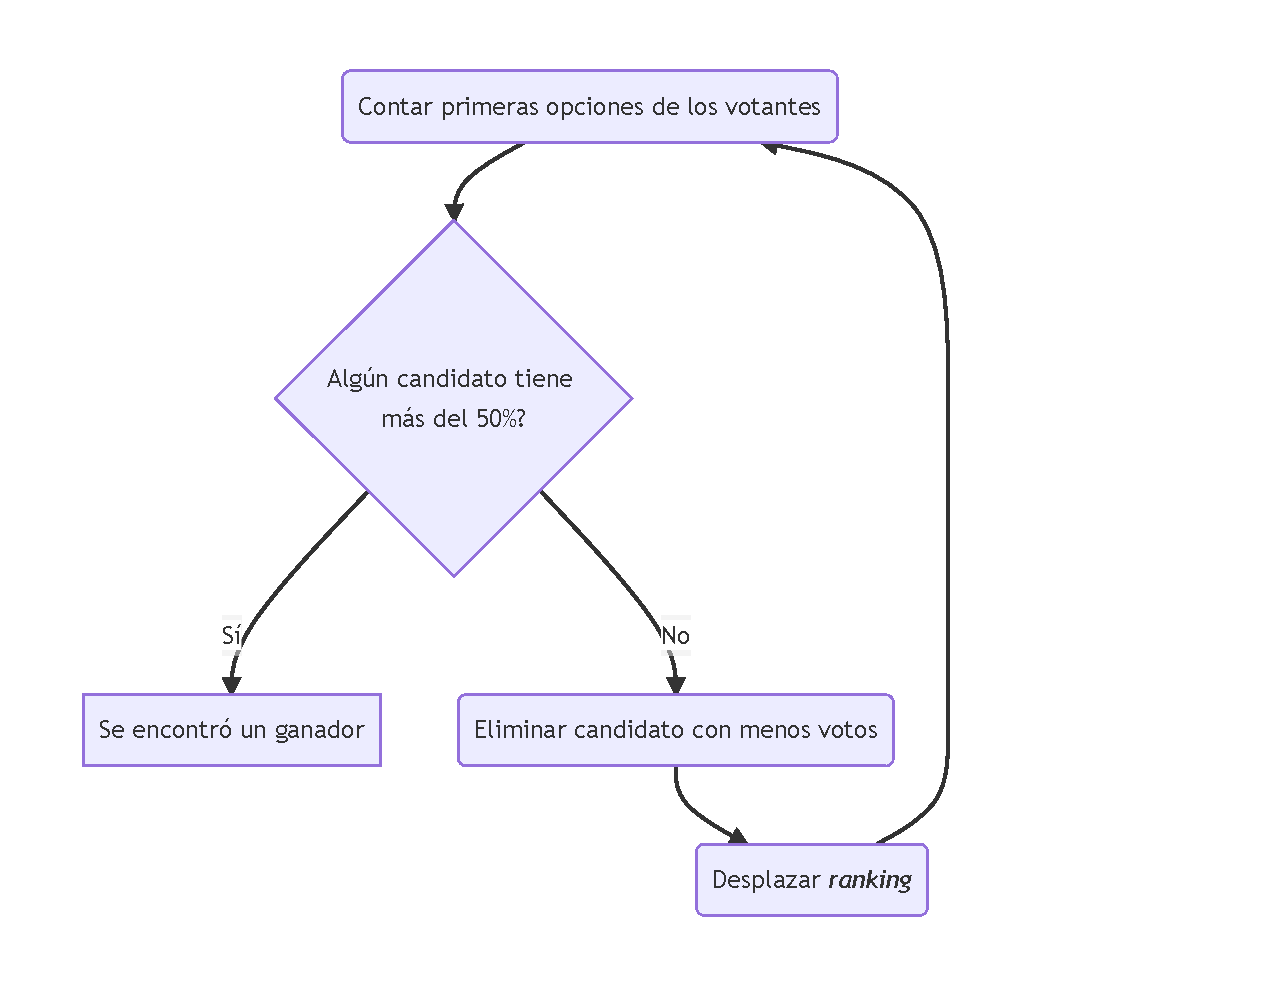
\includegraphics[scale=1.4]{Graphics/irv.pdf}
    \caption{Diagrama de flujo del m\'etodo de desempate instant\'aneo.}
    \label{fig:irv}
\end{figure}

Si m\'as de un candidato posee la menor cantidad de votos, es necesario escoger un m\'etodo de desempate para decidir a cu\'al de ellos eliminar.

\todo[disable,inline]{@TODO esto lleva ejemplo}
\todo[disable,inline]{@TODO decir do'nde se usa esto}